% !TeX spellcheck = hu_HU
% !TeX encoding = UTF-8
\documentclass[11pt,a4paper,oneside]{report}             % Single-side
%\documentclass[11pt,a4paper,twoside,openright]{report}  % Duplex

%\PassOptionsToPackage{chapternumber=Huordinal}{magyar.ldf}
\usepackage{t1enc}
\usepackage[utf8]{inputenc}
\usepackage{amsmath}
\usepackage{amssymb}
\usepackage{enumerate}
\usepackage[thmmarks]{ntheorem}
\usepackage{graphics}
\usepackage{epsfig}
\usepackage{listings}
\usepackage{color}
%\usepackage{fancyhdr}
\usepackage{lastpage}
\usepackage{anysize}
\usepackage[magyar]{babel}
\usepackage{sectsty}
\usepackage{setspace}  % Ettol a tablazatok, abrak, labjegyzetek maradnak 1-es sorkozzel!
\usepackage[hang]{caption}
\usepackage{subcaption}
\usepackage{hyperref}
\usepackage{pdflscape}
\usepackage{fancyvrb}
\usepackage{svg}
\usepackage[pdf]{graphviz}
\usepackage{tikz}
\usetikzlibrary{shapes, calc, positioning}

%--------------------------------------------------------------------------------------
% Main variables
%--------------------------------------------------------------------------------------
\newcommand{\vikszerzo}{Főglein Simon István}
\newcommand{\vikkonzulens}{dr.~Somogyi Péter}
\newcommand{\vikcim}{Grafikus leírónyelvek közös részhalmazának gépi feldolgozása}
\newcommand{\viktanszek}{Irányítástechnika és Informatika Tanszék}
\newcommand{\vikdoktipus}{Önálló laboratórium beszámoló}
%\newcommand{\vikdepartmentr}{Bódis-Szomorú András}

\hypersetup{pdftitle=\vikcim}

%--------------------------------------------------------------------------------------
% Page layout setup
%--------------------------------------------------------------------------------------
% we need to redefine the pagestyle plain
% another possibility is to use the body of this command without \fancypagestyle
% and use \pagestyle{fancy} but in that case the special pages
% (like the ToC, the References, and the Chapter pages)remain in plane style

\pagestyle{plain}
%\setlength{\parindent}{0pt} % áttekinthet?bb, angol nyelv? dokumentumokban jellemz?
%\setlength{\parskip}{8pt plus 3pt minus 3pt} % áttekinthet?bb, angol nyelv? dokumentumokban jellemz?
\setlength{\parindent}{12pt} % magyar nyelv? dokumentumokban jellemz?
\setlength{\parskip}{0pt}    % magyar nyelv? dokumentumokban jellemz?

\marginsize{35mm}{25mm}{15mm}{15mm} % anysize package
\setcounter{secnumdepth}{0}
\sectionfont{\large\upshape\bfseries}
\setcounter{secnumdepth}{2}
\singlespacing
\frenchspacing

%--------------------------------------------------------------------------------------
%	Setup hyperref package
%--------------------------------------------------------------------------------------
\hypersetup{
    bookmarks=true,            % show bookmarks bar?
    unicode=true,             % non-Latin characters in Acrobat’s bookmarks
    pdftitle={\vikcim},        % title
    pdfauthor={\vikszerzo},    % author
    pdfsubject={\vikdoktipus}, % subject of the document
    pdfcreator={\vikszerzo},   % creator of the document
    pdfproducer={Producer},    % producer of the document
    pdfkeywords={keywords},    % list of keywords
    pdfnewwindow=true,         % links in new window
    colorlinks=true,           % false: boxed links; true: colored links
    linkcolor=black,           % color of internal links
    citecolor=black,           % color of links to bibliography
    filecolor=black,           % color of file links
    urlcolor=black             % color of external links
}

%--------------------------------------------------------------------------------------
% Set up listings
%--------------------------------------------------------------------------------------
\lstset{
	basicstyle=\scriptsize\ttfamily, % print whole listing small
	keywordstyle=\color{black}\bfseries\underbar, % underlined bold black keywords
	identifierstyle=, 					% nothing happens
	commentstyle=\color{white}, % white comments
	stringstyle=\scriptsize\sffamily, 			% typewriter type for strings
	showstringspaces=false,     % no special string spaces
	aboveskip=3pt,
	belowskip=3pt,
	columns=fixed,
	backgroundcolor=\color{lightgray},
} 		
\def\lstlistingname{lista}	

%--------------------------------------------------------------------------------------
%	Some new commands and declarations
%--------------------------------------------------------------------------------------
\newcommand{\code}[1]{{\upshape\ttfamily\scriptsize\indent #1}}

% define references
\newcommand{\figref}[1]{\ref{fig:#1}.}
\renewcommand{\eqref}[1]{(\ref{eq:#1})}
\newcommand{\listref}[1]{\ref{listing:#1}.}
\newcommand{\sectref}[1]{\ref{sect:#1}}
\newcommand{\tabref}[1]{\ref{tab:#1}.}

\DeclareMathOperator*{\argmax}{arg\,max}
%\DeclareMathOperator*[1]{\floor}{arg\,max}
\DeclareMathOperator{\sign}{sgn}
\DeclareMathOperator{\rot}{rot}
\definecolor{lightgray}{rgb}{0.95,0.95,0.95}

\author{\vikszerzo}
\title{\viktitle}
\includeonly{
	guideline,%
	project,%
	titlepage,%
	declaration,%
	abstract,%
	introduction,%
	chapter1,%
	chapter2,%
	chapter3,%
	acknowledgement,%
	appendices,%
}
%--------------------------------------------------------------------------------------
%	Setup captions
%--------------------------------------------------------------------------------------
\captionsetup[figure]{
%labelsep=none,
%font={footnotesize,it},
%justification=justified,
width=.75\textwidth,
aboveskip=10pt}

\renewcommand{\captionlabelfont}{\small\bf}
\renewcommand{\captionfont}{\footnotesize\it}

% beszúr egy képet képaláírással és címkével
\newcommand{\kep}[4][1] { % a scale alapértelmezetten 1
	\begin{figure}[h]
		\centering \includegraphics[keepaspectratio, scale=#1]{#2}
		\caption{\centering #3}
		\label{fig:#4}
	\end{figure}
}

%--------------------------------------------------------------------------------------
% Table of contents and the main text
%--------------------------------------------------------------------------------------
\begin{document}
\singlespacing
%% !TeX encoding = UTF-8
% !TeX spellcheck = hu_HU
%--------------------------------------------------------------------------------------
% Rovid formai es tartalmi tajekoztato
%--------------------------------------------------------------------------------------

\footnotesize
\begin{center}
\large
\textbf{\Large Általános információk, a diplomaterv szerkezete}\\
\end{center}

A diplomaterv szerkezete a BME Villamosmérnöki és Informatikai Karán:
\begin{enumerate}
\item	Diplomaterv feladatkiírás
\item	Címoldal
\item	Tartalomjegyzék
\item	A diplomatervező nyilatkozata az önálló munkáról és az elektronikus adatok kezeléséről
\item	Tartalmi összefoglaló magyarul és angolul
\item	Bevezetés: a feladat értelmezése, a tervezés célja, a feladat indokoltsága, a diplomaterv felépítésének rövid összefoglalása
\item	A feladatkiírás pontosítása és részletes elemzése
\item	Előzmények (irodalomkutatás, hasonló alkotások), az ezekből levonható következtetések
\item	A tervezés részletes leírása, a döntési lehetőségek értékelése és a választott megoldások indoklása
\item	A megtervezett műszaki alkotás értékelése, kritikai elemzése, továbbfejlesztési lehetőségek
\item	Esetleges köszönetnyilvánítások
\item	Részletes és pontos irodalomjegyzék
\item	Függelék(ek)
\end{enumerate}

Felhasználható a következő oldaltól kezdődő \LaTeX-Diplomaterv sablon dokumentum tartalma. 

A diplomaterv szabványos méretű A4-es lapokra kerüljön. Az oldalak tükörmargóval készüljenek (mindenhol 2.5cm, baloldalon 1cm-es kötéssel). Az alapértelmezett betűkészlet a 12 pontos Times New Roman, másfeles sorközzel.

Minden oldalon - az első négy szerkezeti elem kivételével - szerepelnie kell az oldalszámnak.

A fejezeteket decimális beosztással kell ellátni. Az ábrákat a megfelelő helyre be kell illeszteni, fejezetenként decimális számmal és kifejező címmel kell ellátni. A fejezeteket decimális aláosztással számozzuk, maximálisan 3 aláosztás mélységben (pl. 2.3.4.1.). Az ábrákat, táblázatokat és képleteket célszerű fejezetenként külön számozni (pl. 2.4. ábra, 4.2 táblázat vagy képletnél (3.2)). A fejezetcímeket igazítsuk balra, a normál szövegnél viszont használjunk sorkiegyenlítést. Az ábrákat, táblázatokat és a hozzájuk tartozó címet igazítsuk középre. A cím a jelölt rész alatt helyezkedjen el.

A képeket lehetőleg rajzoló programmal készítsék el, az egyenleteket egyenlet-szerkesztő segítségével írják le (A \LaTeX~ehhez kézenfekvő megoldásokat nyújt).

Az irodalomjegyzék szövegközi hivatkozása történhet a Harvard-rendszerben (a szerző és az évszám megadásával) vagy sorszámozva. A teljes lista névsor szerinti sorrendben a szöveg végén szerepeljen (sorszámozott irodalmi hivatkozások esetén hivatkozási sorrendben). A szakirodalmi források címeit azonban mindig az eredeti nyelven kell megadni, esetleg zárójelben a fordítással. A listában szereplő valamennyi publikációra hivatkozni kell a szövegben (a \LaTeX-sablon a Bib\TeX~segítségével mindezt automatikusan kezeli). Minden publikáció a szerzők után a következő adatok szerepelnek: folyóirat cikkeknél a pontos cím, a folyóirat címe, évfolyam, szám, oldalszám tól-ig. A folyóirat címeket csak akkor rövidítsük, ha azok nagyon közismertek vagy nagyon hosszúak. Internet hivatkozások megadásakor fontos, hogy az elérési út előtt megadjuk az oldal tulajdonosát és tartalmát (mivel a link egy idő után akár elérhetetlenné is válhat), valamint az elérés időpontját.

\vspace{5mm}
Fontos:
\begin{itemize}
	\item A szakdolgozat készítő / diplomatervező nyilatkozata (a jelen sablonban szereplő szövegtartalommal) kötelező előírás Karunkon ennek hiányában a szakdolgozat/diplomaterv nem bírálható és nem védhető !
	\item Mind a dolgozat, mind a melléklet maximálisan 15 MB méretű lehet !
\end{itemize}

\vspace{5mm}
\begin{center}
Jó munkát, sikeres szakdolgozat készítést ill. diplomatervezést kívánunk !
\end{center}

\normalsize

%% !TeX encoding = UTF-8
% !TeX spellcheck = hu_HU
%--------------------------------------------------------------------------------------
% Feladatkiiras (a tanszeken atveheto, kinyomtatott valtozat)
%--------------------------------------------------------------------------------------
\clearpage
\begin{center}
\large
\textbf{FELADATKIÍRÁS}\\
\end{center}

A feladatkiírást a tanszéki adminisztrációban lehet átvenni, és a leadott munkába eredeti, tanszéki pecséttel ellátott és a tanszékvezető által aláírt lapot kell belefűzni (ezen oldal \emph{helyett}, ez az oldal csak útmutatás). Az elektronikusan feltöltött dolgozatban már nem kell beleszerkeszteni ezt a feladatkiírást.





\pagenumbering{arabic}
\onehalfspacing
% !TeX encoding = UTF-8
% !TeX spellcheck = hu_HU
%--------------------------------------------------------------------------------------
%	The title page
%--------------------------------------------------------------------------------------
\begin{titlepage}
\begin{center}

\includegraphics[width=60mm,keepaspectratio]{figures/BMElogo.png}\\
\vspace{0.3cm}
\textbf{Budapesti Műszaki és Gazdaságtudományi Egyetem}\\
\textmd{Villamosmérnöki és Informatikai Kar}\\
\textmd{\viktanszek}\\[5cm]

\vspace{0.4cm}
{\huge \bfseries \vikcim}\\[0.8cm]
\vspace{0.5cm}
\textsc{\Large \vikdoktipus}\\[4cm]

\begin{tabular}{cc}
 \makebox[7cm]{\emph{Készítette}} & \makebox[7cm]{\emph{Konzulens}} \\
 \makebox[7cm]{\vikszerzo} & \makebox[7cm]{\vikkonzulens}
\end{tabular}

\vfill
{\large \today}
\end{center}
\end{titlepage}



\tableofcontents\vfill
%% !TeX encoding = UTF-8
% !TeX spellcheck = hu_HU
%--------------------------------------------------------------------------------------
% Nyilatkozat
%--------------------------------------------------------------------------------------
\begin{center}
\large
\textbf{HALLGATÓI NYILATKOZAT}\\
\end{center}

Alulírott \emph{\vikszerzo}, szigorló hallgató kijelentem, hogy ezt a beszámolót meg nem engedett segítség nélkül, saját magam készítettem, csak a megadott forrásokat (szakirodalom, eszközök stb.) használtam fel. Minden olyan részt, melyet szó szerint, vagy azonos értelemben, de átfogalmazva más forrásból átvettem, egyértelműen, a forrás megadásával megjelöltem.

Hozzájárulok, hogy a jelen munkám alapadatait (szerző(k), cím, angol és magyar nyelvű tartalmi kivonat, készítés éve, konzulens(ek) neve) a BME VIK nyilvánosan hozzáférhető elektronikus formában, a munka teljes szövegét pedig az egyetem belső hálózatán keresztül (vagy autentikált felhasználók számára) közzétegye. Kijelentem, hogy a benyújtott munka és annak elektronikus verziója megegyezik. Dékáni engedéllyel titkosított diplomatervek esetén a dolgozat szövege csak 3 év eltelte után válik hozzáférhetővé.

\begin{flushleft}
\vspace*{1cm}
Budapest, \today
\end{flushleft}

\begin{flushright}
 \vspace*{1cm}
 \makebox[7cm]{\rule{6cm}{.4pt}}\\
 \makebox[7cm]{\emph{\vikszerzo}}\\
 \makebox[7cm]{hallgató}
\end{flushright}
\thispagestyle{empty}

\vfill
\clearpage
\thispagestyle{empty} % an empty page


%% !TeX encoding = UTF-8
% !TeX spellcheck = hu_HU
%----------------------------------------------------------------------------
% Abstract in hungarian
%----------------------------------------------------------------------------
\chapter*{Kivonat}\addcontentsline{toc}{chapter}{Kivonat}

Jelen dokumentum egy diplomaterv sablon, amely formai keretet ad a BME Villamosmérnöki és Informatikai Karán végző hallgatók által elkészítendő szakdolgozatnak és diplomatervnek. A sablon használata opcionális. Ez a sablon \LaTeX~alapú, a \emph{TeXLive} \TeX-implementációval és a PDF-\LaTeX~fordítóval működőképes.
\vfill

%----------------------------------------------------------------------------
% Abstract in english
%----------------------------------------------------------------------------
\chapter*{Abstract}\addcontentsline{toc}{chapter}{Abstract}

This document is a \LaTeX-based skeleton for BSc/MSc~theses of students at the Electrical Engineering and Informatics Faculty, Budapest University of Technology and Economics. The usage of this skeleton is optional. It has been tested with the \emph{TeXLive} \TeX~implementation, and it requires the PDF-\LaTeX~compiler.
\vfill


% !TeX encoding = UTF-8
% !TeX spellcheck = hu_HU
%----------------------------------------------------------------------------
\chapter*{Bevezető}\addcontentsline{toc}{chapter}{Bevezető}
%----------------------------------------------------------------------------

%A bevezet? tartalmazza a diplomaterv-kiírás elemzését, történelmi el?zményeit, a feladat indokoltságát (a motiváció leírását), az eddigi megoldásokat, és ennek tükrében a hallgató megoldásának összefoglalását.
%
%A bevezet? szokás szerint a diplomaterv felépítésével záródik, azaz annak rövid leírásával, hogy melyik fejezet mivel foglalkozik.

% grafikus keretrendszer, tortn  .. qt gtk, , prior art : miert nem jo. miert csinalod.
% terv. 

% qt, gtk bemutatása
% https://en.wikipedia.org/wiki/Compiler#Front_end
% https://en.wikipedia.org/wiki/Abstract_syntax_tree
% fák ábrája

% TODO: feladat pontosítása
A dolgozat a Qt és GTK felhasználói felület keretrendszerek felületleíró nyelvei közötti átjárhatóságot mutatja be.
Mindkét technológia széleskörűen elterjedt mind a FOSS, mind a kereskedelmi szoftverek körében. A FOSS projektekre jellemző forkolást, továbbfejlesztést segítené a két technológia közötti átjárhatóság. A Qt licencelése jelentősen függ a \textit{The~Qt~Company}-tól, így ha ők a kizárólagos kereskedelmi licenc mellett döntenek \cite{KdeQtOpenSource}, sok projekt bajba kerülhet. A GTK viszont egy tervezése óta szabad szoftverként licencelt GUI keretrendszer, mely alkalmas lehet a Qt helyettesítésére. A Qt, mint keretrendszer pedig alkalmasabb lehet egy komplex projekt megvalósítására, ugyanis az általa biztosított könyvtárak számtalan magasabb absztrakciós szintű osztályt tartalmaznak, ezzel is könnyítve a fejlesztés menetét. Egy fordítóprogram, mely elősegíti a két kezelőfelület-keretrendszer közötti átjárást nagyban segítheti egy projekt más technológiára való átalakítását.

A jelenleg elérhető megoldások nagyon kezdetlegesek, lényegében csak XML $ \rightarrow $ XML és XML $ \rightarrow $ JSON átalakítást tesznek lehetővé, nincs hatékony eljárás a két technológia közötti átjárásra.

% !TeX encoding = UTF-8
% !TeX spellcheck = hu_HU

\chapter{A Qt és GTK keretrendszerek áttekintése}\label{sect:qtgtkoverview}


\section{Bemutatás, rövid történet}
A GTK és a Qt (ejtése mint az angol \textit{cute} szó) széles körben elterjedt GUI eszközkészlet-keretrendszerek. Mindkettővel lehetőség van összetett felhasználói felületek készítésére, a Qt által biztosított osztályok ezen kívül lehetőséget adnak komplex alkalmazások létrehozására is.

A Qt és a GTK története is az 1990-es évekre vezethető vissza. A Qt fejlesztését 1990~nyarán kezdte meg Haavard Nord és Eirik Chambe-Eng, amikor egy ultrahangfelvételek tárolására alkalmas programot fejlesztettek \cite{QtWiki}. Később céget alapítottak, 1994-ben megalakult a Quasar Technologies, ami később Trolltech-ként vált ismertté, manapság pedig a The~Qt~Company nevet viseli. A keretrendszer köré szerveződött cég jól mutatta, hogy a Qt alkotói pénzt szerettek volna keresni a könyvtárral, így a licence nem engedte a szabad terjesztést. Ez először akkor kezdett problémává válni, amikor a KDE -- egy népszerű Linux asztali környezet -- bebiztosította a helyét a túlnyomórészt szabad szoftverekből álló Linuxos világban.

\begin{figure}[h]
	\centering
	\begin{subfigure}{0.4\textwidth}
		\centering
		
\includegraphics[keepaspectratio, scale=0.18]{figures/qt-logo}
	\end{subfigure}
	\hspace{0.075\textwidth}
	\begin{subfigure}{0.3\textwidth}
		\centering
		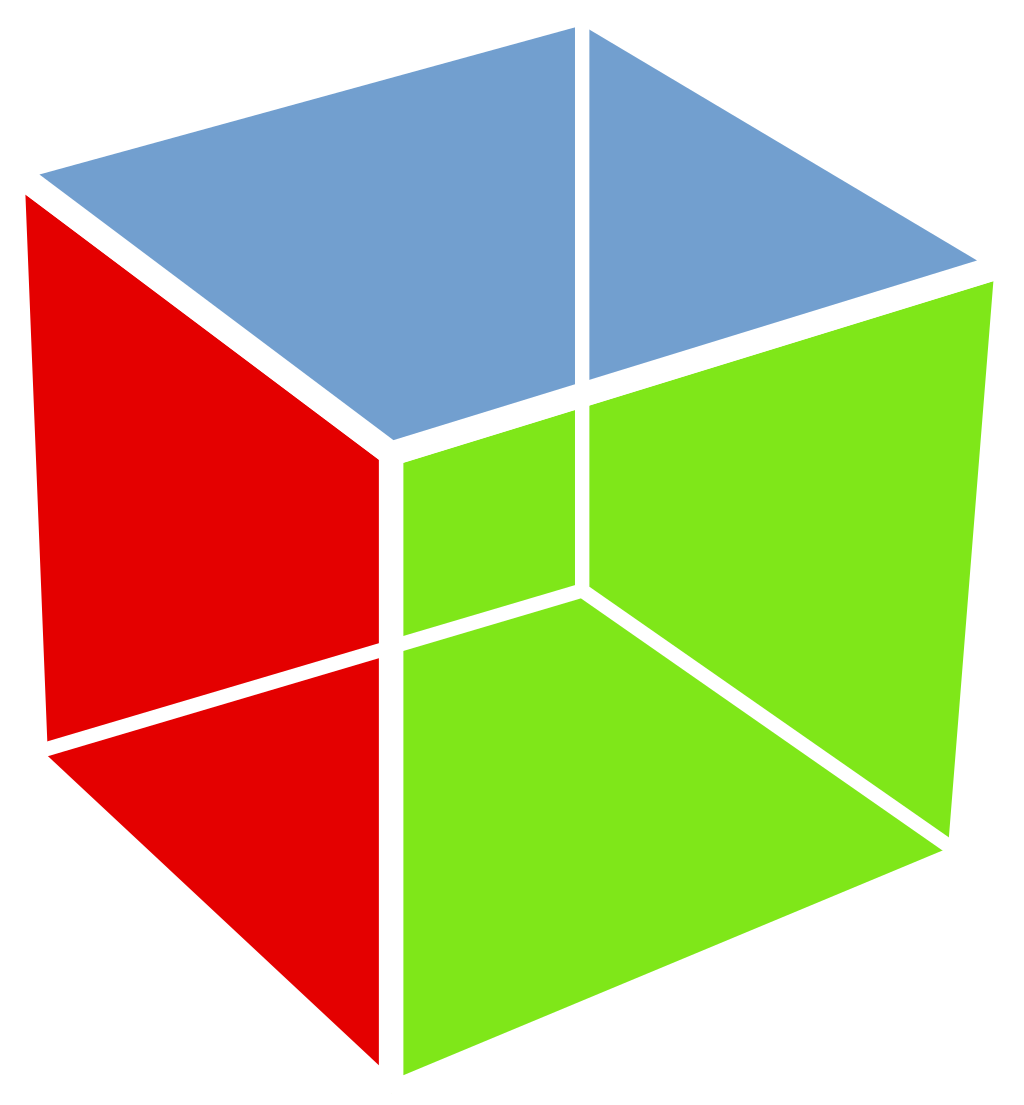
\includegraphics[keepaspectratio, scale=0.11]{figures/gtk-logo}
	\end{subfigure}
	\caption{A Qt és a GTK logója}
	\label{fig:qtgtklogo}
\end{figure}

A GTK történetének kezdete körülbelül 1996-ra tehető, ekkor kezdte meg ugyanis Peter Mattis a keretrendszer fejlesztését \cite{GtkWiki}. A cél a GIMP-hez akkor használt Motif GUI eszközkészlet lecserélése volt (a könyvtár eredeti neve, a GIMP ToolKit is innen ered), amit végül az 1998~nyarán megjelent 1.0-s GIMP verzióval sikerült is véghez vinni.

Mindkét technológia elterjedésében jelentős szerepe volt annak, hogy a '90-es évek végén nagyobb asztali környezetek kezdték el használni mind a Qt, mind a GTK könyvtárakat. A KDE-projekt a Qt egyik legjelentősebb felhasználója és számos változtatással segítik a keretrendszer fejlődését, míg a GNOME asztali környezet fejlesztése a GTK alakulására van nagy hatással. Fontos különbség azonban a fent már említett licencelés problémája: a Qt egy kereskedelmi forgalomban lévő szoftvercsomag, mely néhány kisebb kivétellel (pl. nyílt forráskódú projektek \cite{QtOpenSource}, oktatási célok \cite{QtEdu}) csak licencdíj megfizetése ellenében használható. Ez sokaknak nem tetszett a szabad szoftverekben bővelkedő Unixos világban, így ez is motiválta a GTK korai fázisában a fejlesztést, ugyanis a GTK teljesen szabad licenccel rendelkezik, bárki szabadon felhasználhatja, módosíthatja és terjesztheti is.

\section{Technológiai áttekintés}
% qt xml, qml json, gtk
% gtk builder, qt creator, qt .ui
A Qt elsődleges programozási nyelve a C++, míg a GTK-é a C, bár mindkettőhöz léteznek megoldások más nyelvekkel való együttműködés biztosítására is, mint például Python és C++.

A felhasználói felületek leírásához alapvetően mindkét technológia XML-alapú megoldást használ, bár a Qt esetében lehetőség van a JSON-alapú QML használatára is. A~QML~(Qt~Modeling~Language) egy deklaratív felhasználóifelület-leíró nyelv, melyet a Nokia fejlesztett a Qt projekthez 2009 környékén \cite{QmlWiki}. Előnye az XML-alapú megoldáshoz képest, hogy könnyebben áttekinthető, valamint lehetőséget biztosít JavaScript használatára is, így például a KDE számos alkalmazását folyamatosan portolják -- azaz a funkcionalitás megtartása mellett, általában a felhasználók számára láthatatlan módon megváltoztatják a használt könyvtárakat és a kódbázist -- át a hagyományos C++ és XML technológia helyett a QML-esre (ugyanakkor a QML részei is elérhetőek C++ kódból, például lehetőség van eseménykezelők regisztrálására is).

% TODO: gtk builder vs qt xml-es gui felépítése
% qt a .ui fájlokból a uic segítségével generál ui osztályokat
% gui editorok
A felületleírókban megadott kinézet előállításához a GTK a GTK Builder\footnote{\url{https://docs.gtk.org/gtk3/class.Builder.html}} osztályt használja, míg a Qt a \texttt{uic} segédprogram segítségével generál osztályokat a \texttt{.ui} fájlokból~\cite{qtnotepadtutorial}. Az így generált osztályok a \texttt{Ui} névtéren belül érhetőek el. A felület kódbeli inicializálását az alábbi táblázat mutatja be:
\begin{table}[h]
	\centering
	\begin{tabular}{|c|c|}
		\hline
		Qt & GTK \\
		\hline
		\begin{minipage}{0.35\linewidth}
			\begin{lstlisting}
ui(new Ui::Notepad);
ui->setupUi(this);
			\end{lstlisting}
		\end{minipage}
		&
		\begin{minipage}{0.35\linewidth}
			\begin{lstlisting}
Gtk::Builder::
    new_from_file("ui.glade")
			\end{lstlisting}
		\end{minipage} \\
		\hline
	\end{tabular}
	\label{tab:qtgtkxmlbuild}
	\caption{XML-ben definiált felhasználói felület inicializálása Qt-t és GTK-t használó programokban}
\end{table}

Mivel mindkét szóban forgó keretrendszer lehetőséget biztosít összetett felhasználói felületek létrehozására, és ezek leírása kézzel nagyon körülményes lenne, ezért lehetőség van a felhasználói felületek vizuális összeállítására. Mind a Qt, mind a GTK rendelkezik ilyen programmal: Qt esetében ilyen például a Qt Creator, míg GTK-nál a Glade a legnépszerűbb GUI összeállító program. Bár a \textit{Design} nézet mindkét szerkesztő esetén ugyanazt a célt szolgálja, a két alkalmazás jelentősen eltér egymástól: a Qt Creator egy fejlesztői környezet, mely rendelkezik \textit{Design} nézettel (de emellett lehetőség van pl. C++ forráskód írására, valamint a projekt buildelésére is), a Glade viszont kizárólag a felület összeállításában játszik szerepet. A későbbiekben az ilyen programokkal létrehozott UI-leírók feldolgozására összpontosítunk.

{
\kep[0.35]{figures/qtcreator.png}{A Qt Creator felhasználói felülete design nézetben}{qtcreator}
\kep[0.402]{figures/glade.png}{A Glade felhasználói felülete}{glade}}

\begin{landscape}
	\thispagestyle{empty} % oldalszámozás kihagyása a fektetett oldalon
	\centering % táblázat középre igazítása
	\begin{table}
	\begin{tabular}{|c|c|c|}
		\hline
		QML & Qt XML & GTK XML \\
		\hline
		\begin{minipage}[t]{0.3\linewidth}
			\begin{lstlisting}[numbers=left, xleftmargin=8mm]
QWidget {
    name: "centralWidget"
    QPushButton {
        name: "pushButton"
        geometry: {
            x: 10
            y: 20
            width: 150
            height: 50
        }
        text: "Hello World!"
    }
}
			\end{lstlisting}
		\end{minipage}
		&
		\begin{minipage}[t]{0.3\linewidth}
			\begin{lstlisting}[language=xml, numbers=left, xleftmargin=8mm]
<widget class="QWidget"
	    name="centralWidget">
  <widget class="QPushButton"
          name="pushButton">
    <property name="geometry">
      <rect>
        <x>10</x>
        <y>20</y>
        <width>150</width>
        <height>50</height>
      </rect>
    </property>
    <property name="text">
      <string>Hello World!</string>
    </property>
  </widget>
</widget>
			\end{lstlisting}
		\end{minipage}
		&
		\begin{minipage}[t]{0.3\linewidth}
			\begin{lstlisting}[language=xml, numbers=left, xleftmargin=8mm]
<object class="GtkFrame">
  <child>
    <object class="GtkButton"
        id="pushButton">
      <property name="label"
          translatable="yes">
          Hello World!
        </property>
        <property name="name">
          pushButton
        </property>
    </object>
  </child>
</object>
			\end{lstlisting}
		\end{minipage} \\
		\hline
	\end{tabular}
	\caption{A QML, Qt XML és a GTK XML felépítésének összehasonlítása}
	\label{tab:sourcecomparison}
	\end{table}
\end{landscape}

% !TeX encoding = UTF-8
% !TeX spellcheck = hu_HU

\chapter{Fordítóprogramok}

\section{Fordítóprogramok bemutatása}
A fordítóprogramok olyan számítógépes szoftverek, amelyek egy adott programozási nyelven írt programot képesek egy másik programozási nyelvre, vagy számítógépek által értelmezhető, futtatható gépi kódra átalakítani.

\section{Fordítóprogramok architektúrája}
% !TeX encoding = UTF-8
% !TeX spellcheck = hu_HU

\chapter{Saját munka bemutatása}

A fordítóprogramok nagyon komplex szoftverek. A legismertebb C/C++ fordítóprogram talán a GCC (GNU Compiler Collection), amely óriási kódbázissal rendelkezik, 2019-ben~körülbelül 15~millió sort tartalmaztak a forrásállományai \cite{GccWiki}. Természetesen egy GCC szintű fordítóprogram számos olyan funkcióval rendelkezik, mely a több, mint 36 évnyi fejlesztésből és a projekt léptékéből adódik, ilyen például a többféle programozási nyelv támogatása, valamint a fejlett optimalizációs megoldások. Ezen funkciók közül jó néhányat egy felhasználóifelület-leíró nyelveket támogató fordítóprogramnak nem szükséges biztosítania, és mivel az Önálló laboratórium tárgy választott témájának keretében a fordítóprogramok felépítésének és készítésének, valamint a programozási nyelvek konstrukcióinak mélyebb megismerése állt a középpontban, így elsősorban ezekre fektettem nagy hangsúlyt az irodalomkutatás során, továbbá ilyen területekre fogok összpontosítani a fordítóprogramom implementálása alatt is.



\section{Feladat specifikációja}
Az Önálló laboratórium projekt keretében egy úgynevezett \textit{source-to-source} fordítót készítek. Amint azt \az{ \sectref{compilerintro}}.~fejezetben ismertettem, az ilyen fordítók forrásfájlok közötti fordításra alkalmasak, azaz a bemenetként kapott fájlokból nem futtatható kódot generálnak, hanem egy másik nyelvre fordítják át azt. A projektfeladat keretében létrehozott fordító \az{\sectref{qtgtkoverview}}.~fejezetben és \az{\tabref{sourcecomparison}}~táblázatban bemutatott keretrendszerek felületleíró nyelveinek egy részhalmazát képes a QML, Qt XML és GTK XML között átalakítani.

\subsubsection{Támogatott formátumok}
A fentiek értelmében a program a tárgyalt két keretrendszer XML- és JSON-alapú nyelvei között teszi lehetővé a fordítást. Ennek megfelelően a bemeneti fájloknak az adott platform specifikációit kielégítően kell felépülniük, a kiterjesztésüknek pedig egyértelműen meghatározhatóvá kell tenni a forrásfájl típusát (azaz a \texttt{.ui} (Qt XML), \texttt{.qml} és \texttt{.glade} (GTK XML) hármas közül kell kikerülnie). A program ez alapján tudja eldönteni, hogy melyik értelmező (parser) modult kell meghívnia.

\subsection{Közös részhalmaz meghatározása} \label{sect:featuresubset}
Mivel a feladat során a hangsúly a fordítóprogramok felépítésének és működésének megismerésén van, továbbá az ismertetett keretrendszerek rengeteg felhasználásiterület-specifikus komponenssel rendelkeznek, melyeknek gyakran nincs is pontos megfelelője a másik keretrendszerben, ezért a fordítandó komponenseket az alapvető felhasználói felületi elemekre korlátoztam. Így végül egyszerű konténerek, gombok és beviteli mezők fordítására van lehetőség a programban.

A megfelelő részhalmaz kiválasztása a vártnál nagyobb kihívást jelentett, ugyanis sok felületi elem teljesen más tulajdonságokkal van ellátva a másik könyvtárhoz képest. Ilyen például, hogy GTK-ban alapvetően nem adható meg egy gomb pontos pozíciója és mérete, hanem kitölti a szülőkomponensben rendelkezésre álló helyet. Emiatt a gombok méretének beállítására csak akkor van lehetőség, ha a fordítás a két Qt-fájltípus, a \texttt{.ui} és a \texttt{.qml} között valósul meg (a fordítás iránya felcserélhető).

A programban lehetőség van a bemeneti fájl struktúrájának vizuális megjelenítésére is. Ehhez kimeneti fájlként egy \texttt{.svg} kiterjesztésű fájlt kell megadni. Ekkor a program az első két fázisban (ld. következő alfejezet) ugyanúgy viselkedik, mint általános esetben, de a kódgenerálási lépés során felületleíró fájl helyett egy vektorgrafikus állományt készít, mely egy irányított gráf formájában mutatja be a bemeneti fájl felépítését.

\section{A program felépítése és működése}
% TODO: dir ábra
\kep[0.67]{figures/dirtree.pdf}{A program architektúrája}{mycompilerarch}

Ahogy arról már \az{\sectref{compilerarch}} fejezetben is szó volt, a fordítóprogramok általában háromrétegűek, és a rétegek jól elkülöníthetőek. A munkám során törekedtem ezen architektúra követésére: külön egységbe kerültek a forrásnyelvelemző, a belső reprezentáció és a kódgenerálás forrásfájljai. Ezeken túl még röviden kitérek arra is, hogy a felhasználók hogyan használhatják a programot a parancssoron keresztül.


\subsection{Parancssori interfész}
A felhasználók parancssoron keresztül indíthatják el a programot, itt van lehetőség a forrás- és kimeneti fájlok elérési útjának megadására. A megadott paramétereket a Python által biztosított \texttt{ArgumentParser} osztály segítségével dolgozzuk fel. A megadott paraméterek helyességét is ellenőrizzük, ez látható az alábbi kódrészleten:

\begin{table}[h]
	\centering
	\begin{tabular}{c}
		\begin{minipage}[c]{0.92\linewidth}
			\begin{lstlisting}[numbers=left, frame=single, language=Python, caption={A parancssori argumentumok helyességét ellenőrző függvény}, captionpos=b]
INPUT_FORMATS = ["qml", "glade", "ui"]
OUTPUT_FORMATS = ["qml", "glade", "ui", "svg"]
				
def validate_command(args):
    return os.path.isfile(args.source_file) \
        and os.path.splitext(args.source_file)[1][1:] in INPUT_FORMATS \
        and os.path.splitext(args.destination_file)[1][1:] in OUTPUT_FORMATS
			\end{lstlisting}
		\end{minipage}
	\end{tabular}
\end{table}

%TODO: Belső reprezentáció objektumorientált
% TODO: kép a tree-ről

\subsection{Front end}
A front end feladata, hogy ellenőrizze és értelmezze a kapott forrásfájlokat. A projekten belül az ide tartozó kódrészek a \textit{parsers} mappában kaptak helyet.

Ezeknek a moduloknak a felelőssége, hogy a megadott bemeneti fájlokat beolvassák, szintaktikailag ellenőrizzék és felépítsék belőle a middle end által használt abszrakt belső reprezentációt, az Absztrakt Szintakszisfát (Abstract Syntax Tree, AST). Ennek a feladata, hogy az alkotó csomópontok elemeit -- esetünkben a vezérlőelemeket -- a be- és kimeneti nyelvtől függetlenül reprezentálja.

\subsection{Middle end}
Esetemben a middle end feladata egy egységes reprezentáció biztosítása a felhasználói felület elemei számára, hogy azok a forrás- és célplatformtól függetlenül legyenek kezelhetőek a programon belül. Ezt objektumorientáltan, Python osztályok segítségével valósítottam meg.

\kep[1]{figures/uml.pdf}{A belső reprezentáció felépítése}{fig:ir}

\subsection{Back end}
A backend feladata a kódgenerálás. Ehhez paraméterként kapja a korábbi lépésekben előállított absztrakt szintakszisfát, és ezek tulajdonságainak ismeretében állítja elő a célnyelv forrásállományait. Ezekhez általában valamilyen sablont használ.


\subsection{Hibakezelés}
A program implementálása során nagy hangsúlyt fektettem a hibakezelésre. Ez igaz mind a felhasználói parancsok értelmezésére, mind a program belső működésére, ezzel is könnyítve a későbbi bővítést és növelve a hibakeresés hatékonyságát.




\begin{table}[h]
	\centering
	\begin{tabular}{c}
		\begin{minipage}[c]{0.65\linewidth}
			\begin{lstlisting}[numbers=left, frame=single, language=xml, caption={Hibaüzenetet előidéző kódrészlet}, captionpos=b]
  <item row="1" column="0">
    <widget class="QTimeEdit" name="timeEdit"/>
  </item>
			\end{lstlisting}
		\end{minipage}
	\end{tabular}
\end{table}

\begin{table}[h]
	\centering
	\begin{tabular}{c}
		\begin{minipage}[c]{0.65\linewidth}
			\begin{lstlisting}[numbers=left, frame=single, caption={A fenti kódrészletre kapott hibaüzenet}, captionpos=b]
 python3 main.py --from mainwindow.ui --to qmlout.qml

 Unsupported widget type 'QTimeEdit' in input file.
			\end{lstlisting}
		\end{minipage}
	\end{tabular}
\end{table}
%Exceptionök, nem várt node-ok, programindítás paraméterei


% köztes reprezentáció a különböző bemenetek alapján a middle-endre
% xml, qml gráf rajzolása dotml schema (DOT) graphviz XML; svg generálása?

% gtk hw qt hw doxygen class hiersh

% szintaxisfa rajzolása

% generált felületekről képek

\section{Jelenlegi limitációk, továbbfejlesztési lehetőségek}
A program jelenleg a Qt és a GTK eszközkészletének csak egy kis részét fedi le, így könnyű olyan funkciót vagy felhasználóifelületi elemet találni, amelynek implementálásával érdemes lehet foglalkozni a jövőben.

Mivel mindkét könyvtár többféle megoldást kínál a vezérlőelemek felhasználói felületen való elrendezésére, ezért kézenfekvőnek tűnhet a különböző konténerosztályok feldolgozásának támogatását kitűzni következő mérföldkőként. Ehhez a motivációt növeli, hogy az összetettebb felhasználói felületek mind használnak ilyen osztályokat, általában többet is, egymásba ágyazva. A program jelenleg nem támogatja teljeskörűen az ilyen felületeket: GTK és Qt közötti fordításnál például bizonyos bemenetek esetén előfordulhat, hogy az elemek nem az elvárt pozícióba kerülnek. Ennek legfőbb oka, hogy a GTK-s vezérlők a Qt-nál látottakkal ellentétben alapértelmezetten kitöltik a számukra rendelkezésre álló helyet, és ezt csak különböző konténerek bevezetésével lehet felülírni, ami Qt-ban látottakhoz képest sokkal összetettebb logikát igényel a programban.

A másik fő irány, amiben a program továbbfejlesztésre szorul, az az elérhető vezérlők számának növelése. Ahogy arra \az{\sectref{featuresubset}} alfejezetben kitértem, a program jelenlegi állapotában csak néhány alapvető felhasználóifelületi elemet támogat, ami jelentősen korlátozza a felhasználási körét. Új vezérlők hozzáadása a program jelenlegi felépítése mellett már sokkal könnyebb, ugyanis már sok, az új elemek kezeléséhez szükséges megoldásra szükség volt a jelenlegi állapot eléréséhez is, ezek pedig a program moduláris mivoltából adódóan könnyen újrafelhasználhatóak. Ilyen megoldásnak tekinthető például a belső reprezentáció alaposztálya, az \texttt{AstBase}, melyből egy új osztályt leszármaztatva vehetjük fel a kívánt felületi elemet a programba. Emellett rendelkezésre állnak már egyes adatstruktúrák és fabejáró függvények a jövőbeni munka megkönnyítésére.

%% !TeX encoding = UTF-8
% !TeX spellcheck = hu_HU
%----------------------------------------------------------------------------
\chapter*{Köszönetnyilvánítás}\addcontentsline{toc}{chapter}{Köszönetnyilvánítás}
%----------------------------------------------------------------------------

Ez nem kötelező, akár törölhető is. Ha a szerző szükségét érzi, itt lehet köszönetet nyilvánítani azoknak, akik hozzájárultak munkájukkal ahhoz, hogy a hallgató a szakdolgozatban vagy diplomamunkában leírt feladatokat sikeresen elvégezze. A konzulensnek való köszönetnyilvánítás sem kötelező, a konzulensnek hivatalosan is dolga, hogy a hallgatót konzultálja.


%\listoffigures\addcontentsline{toc}{chapter}{Ábrák jegyzéke}
%\listoftables\addcontentsline{toc}{chapter}{Táblázatok jegyzéke}

\bibliography{mybib}
\addcontentsline{toc}{chapter}{Irodalomjegyzék}
\bibliographystyle{plain}

%% !TeX encoding = UTF-8
% !TeX spellcheck = hu_HU
%----------------------------------------------------------------------------
\appendix
%----------------------------------------------------------------------------
\chapter*{Függelék}\addcontentsline{toc}{chapter}{Függelék}
\setcounter{chapter}{6}  % a fofejezet-szamlalo az angol ABC 6. betuje (F) lesz
\setcounter{equation}{0} % a fofejezet-szamlalo az angol ABC 6. betuje (F) lesz
\numberwithin{equation}{section}
\numberwithin{figure}{section}
\numberwithin{lstlisting}{section}
%\numberwithin{tabular}{section}








\label{page:last}
\end{document}
